\documentclass[10pt,a4paper,twocolumn]{article}

% Packages used (preferably in alphabetical order to identify and avoid duplicates
\usepackage{amsmath,amssymb}
\usepackage{balance}
\usepackage{booktabs}
\usepackage{caption}
\usepackage[margin=17mm]{geometry}
\usepackage{graphicx}
	\graphicspath{
		{./}
		{../graphics/}
	}
\usepackage{hyperref}
\hypersetup{
  	bookmarks=true,         % show bookmarks bar?
    unicode=false,          % non-Latin characters in Acrobat's bookmarks
    pdftoolbar=true,        % show Acrobat's toolbar?
    pdfmenubar=true,        % show Acrobat's menu?
    pdffitwindow=true,      % page fit to window when opened
    pdftitle={Multi-agent systems}, 	% title
    pdfauthor={},      		% author
    pdfsubject={},  		% subject of the document
    pdfnewwindow=true,      % links in new window
    pdfkeywords={},			% list of keywords
    colorlinks=true,   		% false: boxed links; true: colored links
    linkcolor=blue,        	% color of internal links
    citecolor=blue, 		% color of links to bibliography
    filecolor=blue,      	% color of file links
    urlcolor=blue           % color of external links
}	
\usepackage{lipsum}
\usepackage{microtype}     % improves justification
\usepackage[numbers,sort&compress]{natbib}
	\bibliographystyle{apalike2}

% Title information
\title{Ecological Resilience in Marine Environments: Modeling Shipwreck Impacts}
\author{
  Toon Sterckx \\
  {\small KU Leuven} \\
  \texttt{toon.sterckx@student.kuleuven.be}
  \and
  Katri Kyllikki Aalto-Setälä \\
  {\small KU Leuven} \\
  \texttt{katrikyllikki.aalto-setaelae@student.kuleuven.be}
  \and
  Gustave Mougenot \\
  {\small KU Leuven} \\
  \texttt{gustave.mougenot@student.kuleuven.be}
}
\date{05.06.2026}

\begin{document}
\maketitle

\begin{abstract}
Shipwrecks introduce both short-term ecological disturbance and long-term habitat complexity in marine environments. This paper presents an agent-based model to study the behavioral sensitivity of fish populations to such disturbances. Fish agents interact with food, predators, and a dynamic environment in which a shipwreck event acts as an intervention, introducing mortality, pollution, and shelter. We systematically vary behavioral parameters, specifically shelter-seeking and schooling tendencies, to analyze their impact on system outcomes. Results(placeholder) show that increased shelter-seeking behavior increases short-term mortality but slows long-term population improvement, revealing a trade-off between safety and resource acquisition. These findings highlight how small changes in individual behavior can lead to significantly different ecosystem-level dynamics, demonstrating the value of agent-based modelling for studying ecological resilience.
\end{abstract}

\section{Introduction}
Approximately three million shipwrecks exist in the bottom of the ocean world widely. Shipwrecks arise from catastrophic events in navigable water body. The events can be natural disasters, human induced accidents, conflict and naval warfare. A ship can also be intentionally sunk (e.g. artificial reefs) which makes it an abandonment. After a while, years, submerged wrecks become part of the "site formation process". Paxton et al. (2024) \cite{ShipsPaxton} concluded these physical, chemical and biological processes interact with each other and that affects also the underwater ecology.  While the shipwrecks can increase habitat complexity over time, they initially disrupt marine ecosystems through pollution, reduced water quality, and altered resource distribution. This interaction between short-term disturbance and long-term habitat change makes shipwrecks a useful case for studying ecological resilience, which has been studied by Paxton et al.\cite{ShipsPaxton} This project models a small, simple, localized marine environment to explore how a shipwreck could affect food availability, predation risk, and fish population dynamics over short and long time scales. The model is deliberately abstract, focusing on essential ecological mechanisms rather than replicating a specific real ecosystem.

\section{Introduction}

Approximately three million shipwrecks are distributed across the world’s oceans. While shipwrecks arise from events such as natural disasters, accidents, or warfare, they can also be intentionally created as artificial reefs. Over time, submerged wrecks become integrated into marine ecosystems through physical, chemical, and biological processes \citep{ShipsPaxton}.

Shipwrecks exhibit a dual ecological effect. In the short term, they disrupt ecosystems through pollution, reduced water quality, and altered resource distribution. In the long term, however, they may increase habitat complexity and serve as shelters for marine species. This combination of disturbance and habitat creation makes shipwrecks a compelling case for studying ecological resilience.

Understanding such dynamics requires modelling individual behaviour and local interactions. Agent-based modelling (ABM) is well suited for this purpose, as it captures how simple behavioural rules at the individual level lead to emergent system-level patterns.

This study develops a simplified agent-based model of a marine ecosystem to investigate how fish populations respond to a shipwreck disturbance. We specifically analyse the behavioural sensitivity of the system with respect to shelter-seeking and schooling tendencies.

\section{Background}
Here the discussion on other papers.
\subsection{Effects caused by ship sinking}
Consoli et al., through their multivariate analysis of shipwrecks, demonstrated that areas close to the wrecks exhibit higher species richness and abundance compared to nearby soft seabed regions. This finding suggests that shipwrecks function as artificial reefs, drawing in groups of fish and contributing to increased diversity within the local fish community.\cite{effectShipwrecks}
Shipwrecks introduce artificial structures that serve as underwater habitats for a wide range of organisms, from microscopic life to large marine species. Some wrecks are even considered distinctive biodiversity hotspots. They provide shelter for various fish species, including small, hidden species that inhabit crevices, larger bottom-dwelling fish that move around the wreck, and schooling baitfish and predators that occupy the surrounding water column. When ships sink, they settle onto existing natural habitats. \cite{ShipsPaxton}

Establishing a monitoring network of shipwrecks would create valuable opportunities to examine ecological concepts such as island biogeography, succession, disturbance, and other ecosystem processes across both time and space. For instance, the order and timing of ecological succession on shipwrecks remain poorly understood and could be clarified through more systematic and intensive observation.\cite{ShipsPaxton}


\subsection{Prey and predator}
 
How is the ship wreck studied in other papers?
- ship wreck, time, causes, effects on the submarine environment
Prey and predator logic, over all history
-> mention the agent logic in anylogic
\subsection{Agent based systems}

Agent-Based Modeling (ABM) is a computational methodology used to analyze systems composed of diverse, interacting agents. The behavioral rules assigned to artificial agents are typically simpler than those governing real-world actors. 
However, despite this simplicity at the individual level, the combination of these micro-level behaviors can produce complex emergent dynamics that cannot be fully understood by examining agents in isolation.\cite{ar:GallegatiEtAl2024}
In most agent-based models, one or more categories of agents are defined, each with distinct characteristics related to their resources and patterns of behavior and interaction, often within localized networks. Additionally, artificial agents can modify their behavior by selecting from a predefined set of action rules, allowing them to adapt to changes in their environment.\cite{ar:GallegatiEtAl2024}

 The term Agent-Based Modeling refers to a class of modelling approaches designed to study systems whose overall behavior emerges from ongoing interactions among heterogeneous entities. These systems range from the particle systems studied in physics to integrated human-natural systems in socioecology. In this context, agents are broadly understood as software entities capable of representing individuals, social groups, institutions, biological organisms, or even physical objects.\cite{ar:GallegatiEtAl2024}




\subsection{Target Phenomenon and Emergence}
The target phenomenon that this project examines is the emergent change in fish population size, environment stability, and survival patterns following a shipwreck. We distinguish explicitly between short- and long-term effects. In the short term, first impact, pollution and food disruption are expected to increase mortality. After xx time the fishes begin to use the wreck as a shelter and the food availability normalizes. Population-level outcomes emerge from individual fish decisions about movement, feeding, and shelter use, linking environmental disturbance to ecosystem-scale dynamics.

\section{Background}

\subsection{Shipwreck ecology}

Shipwrecks introduce artificial structures that significantly alter marine ecosystems. Empirical studies show that areas surrounding wrecks often exhibit higher species richness and abundance compared to nearby soft seabed environments, indicating their role as artificial reefs \citep{effectShipwrecks}. These structures provide shelter, attract prey species, and create new ecological niches.

At the same time, shipwrecks act as ecological disturbances, particularly immediately after sinking. They can introduce pollution, reduce water quality, and disrupt existing habitats \citep{ShipsPaxton}. Over time, however, ecosystems reorganise through physical, chemical, and biological processes, leading to increased habitat complexity and potential biodiversity gains.

This dual effect highlights key ecological mechanisms relevant for modelling: an initial mortality shock, temporary resource disruption, and the gradual introduction of shelter.

\subsection{Predation and resource dynamics}

Marine ecosystems are strongly shaped by predator-prey interactions and resource availability. Fish survival depends on balancing food-seeking behaviour with avoidance of predation risk. Environmental changes, such as the introduction of shelter or pollution, can alter this balance by affecting both food distribution and safe movement within the habitat.

These interactions are inherently local and dynamic, making them suitable for representation using individual-based approaches.

\subsection{Agent-based modelling and behavioural sensitivity}

Agent-based modelling (ABM) is a computational approach for studying systems composed of interacting autonomous agents. Although individual behavioural rules are typically simple, their interaction can produce complex emergent dynamics that cannot be understood by analysing agents in isolation \citep{ar:GallegatiEtAl2024}.

A key strength of ABM is its ability to test behavioural sensitivity: how variations in individual decision rules affect system-level outcomes. Small changes in behaviour, such as increased risk aversion or preference for shelter, can lead to significantly different population trajectories.

\subsection{Target phenomenon and model abstraction}

This study focuses on the emergent dynamics of fish populations following a shipwreck disturbance. Based on the literature, we abstract the system to three core mechanisms:
\begin{itemize}
    \item short-term disturbance (mortality and pollution)
    \item long-term habitat formation (shelter)
    \item behavioural trade-offs between safety and resource acquisition
\end{itemize}

By isolating these mechanisms, the model provides a controlled setting to analyse how behavioural assumptions influence ecological resilience.

\section{Method}

We develop a minimal agent-based model to study the impact of a shipwreck disturbance on fish population dynamics. The model focuses on essential mechanisms and their behavioural sensitivity rather than ecological realism.

\subsection{Model overview}

The simulation follows a before–after design. In the baseline phase, the fish population evolves under stable conditions until a dynamic equilibrium is reached. At time $t = T_w$, a shipwreck event is introduced, after which the system transitions to a new equilibrium.

Multiple simulation runs are performed while systematically varying behavioural parameters. Key performance indicators include population size, survival rate, and recovery time.

\subsection{Agents}

\subsubsection{\texttt{A\_Fish}}

Fish agents represent individual organisms with internal state variables such as energy and age. They move through space, consume food, reproduce, and die based on their state.

Fish behaviour is modelled using a behaviour-based statechart (Figure~\ref{fig:fishAgent}). At each time step, fish perceive their local environment (food, predators, shelter) and select actions accordingly. Behavioural rules include:
\begin{itemize}
    \item food-seeking (movement towards nearby resources),
    \item predator avoidance,
    \item shelter-seeking,
    \item schooling (movement towards nearby fish),
    \item reproduction when sufficient energy is available.
\end{itemize}

Two key behavioural parameters are varied:
\begin{itemize}
    \item shelter preference,
    \item schooling tendency.
\end{itemize}

\begin{figure}[h]
    \centering
    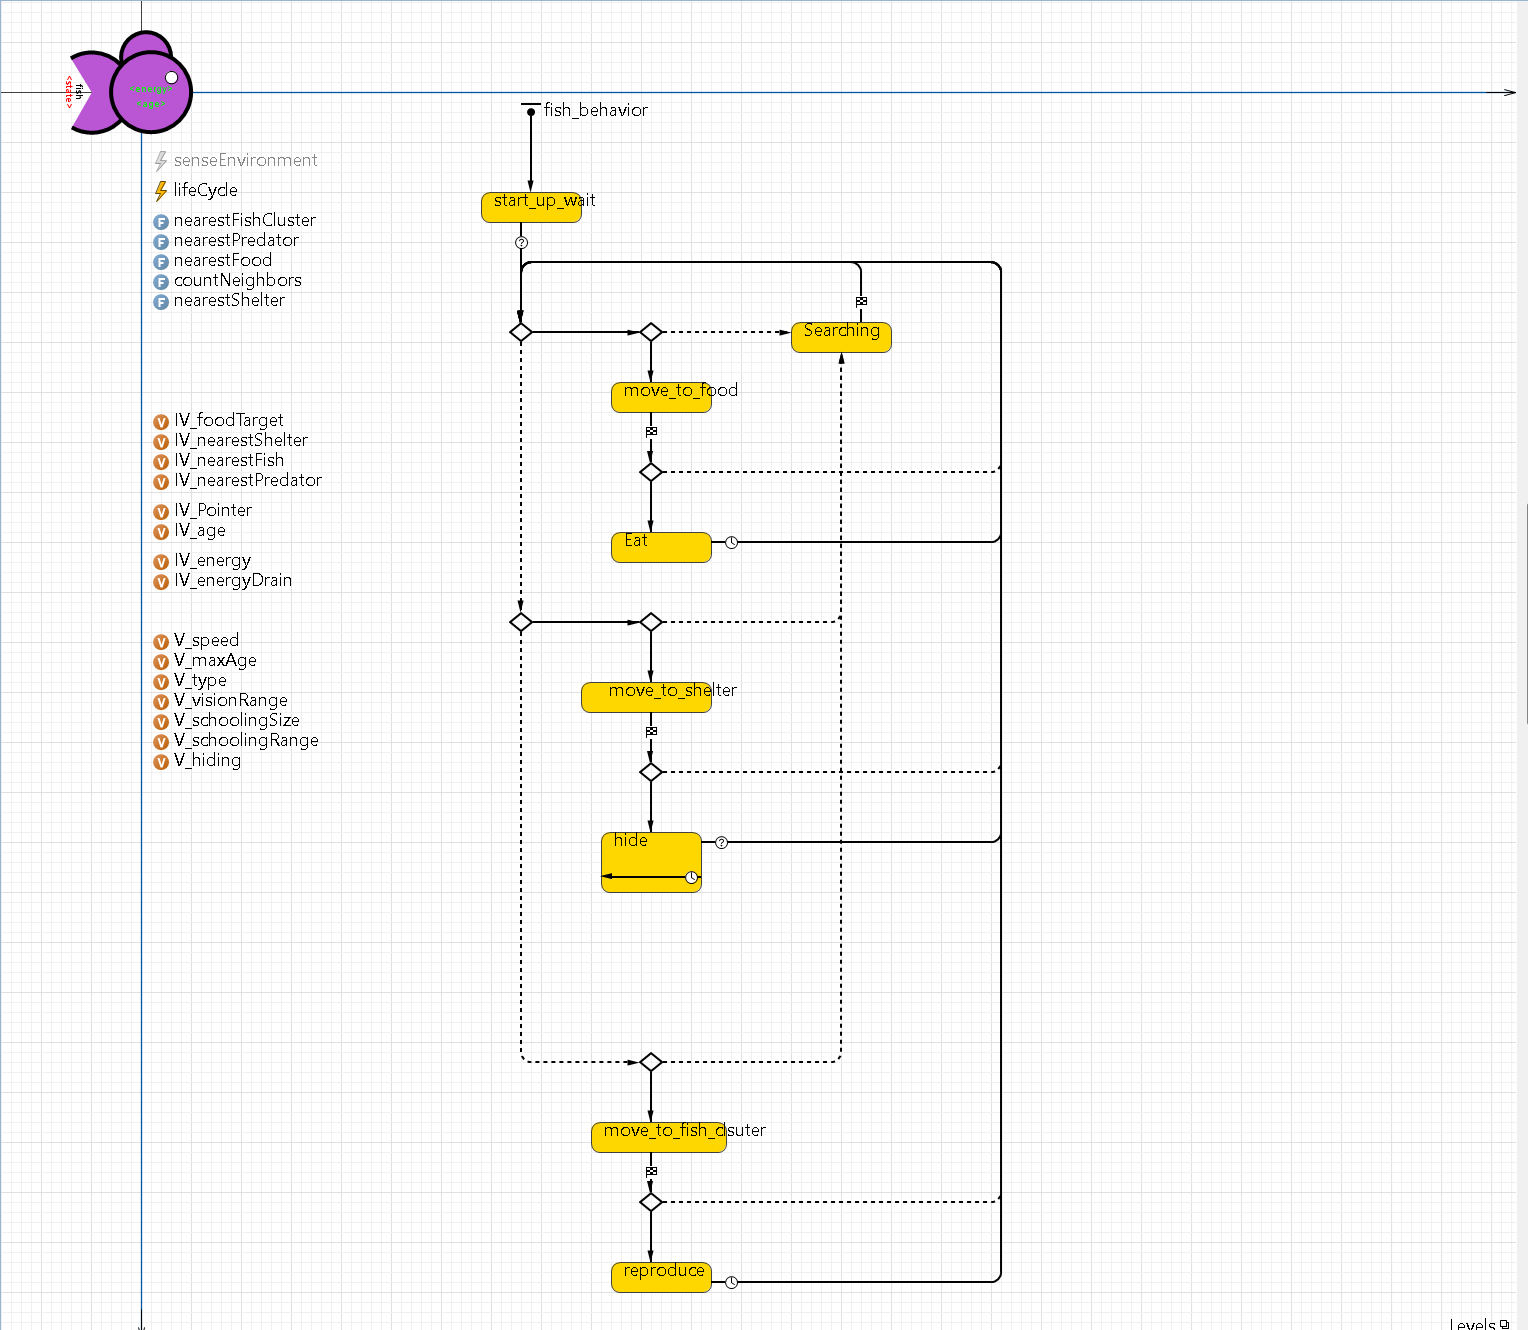
\includegraphics[width=0.9\columnwidth]{A_fish.png}
    \caption{Fish agent statechart}
    \label{fig:fishAgent}
\end{figure}

\subsubsection{\texttt{A\_Predator}}

Predators are modelled as agents that move through the environment and consume fish upon encounter. Predator behaviour is driven by simple hunting rules and internal energy dynamics (Figure~\ref{fig:predatorAgent}).

\begin{figure}[h]
    \centering
    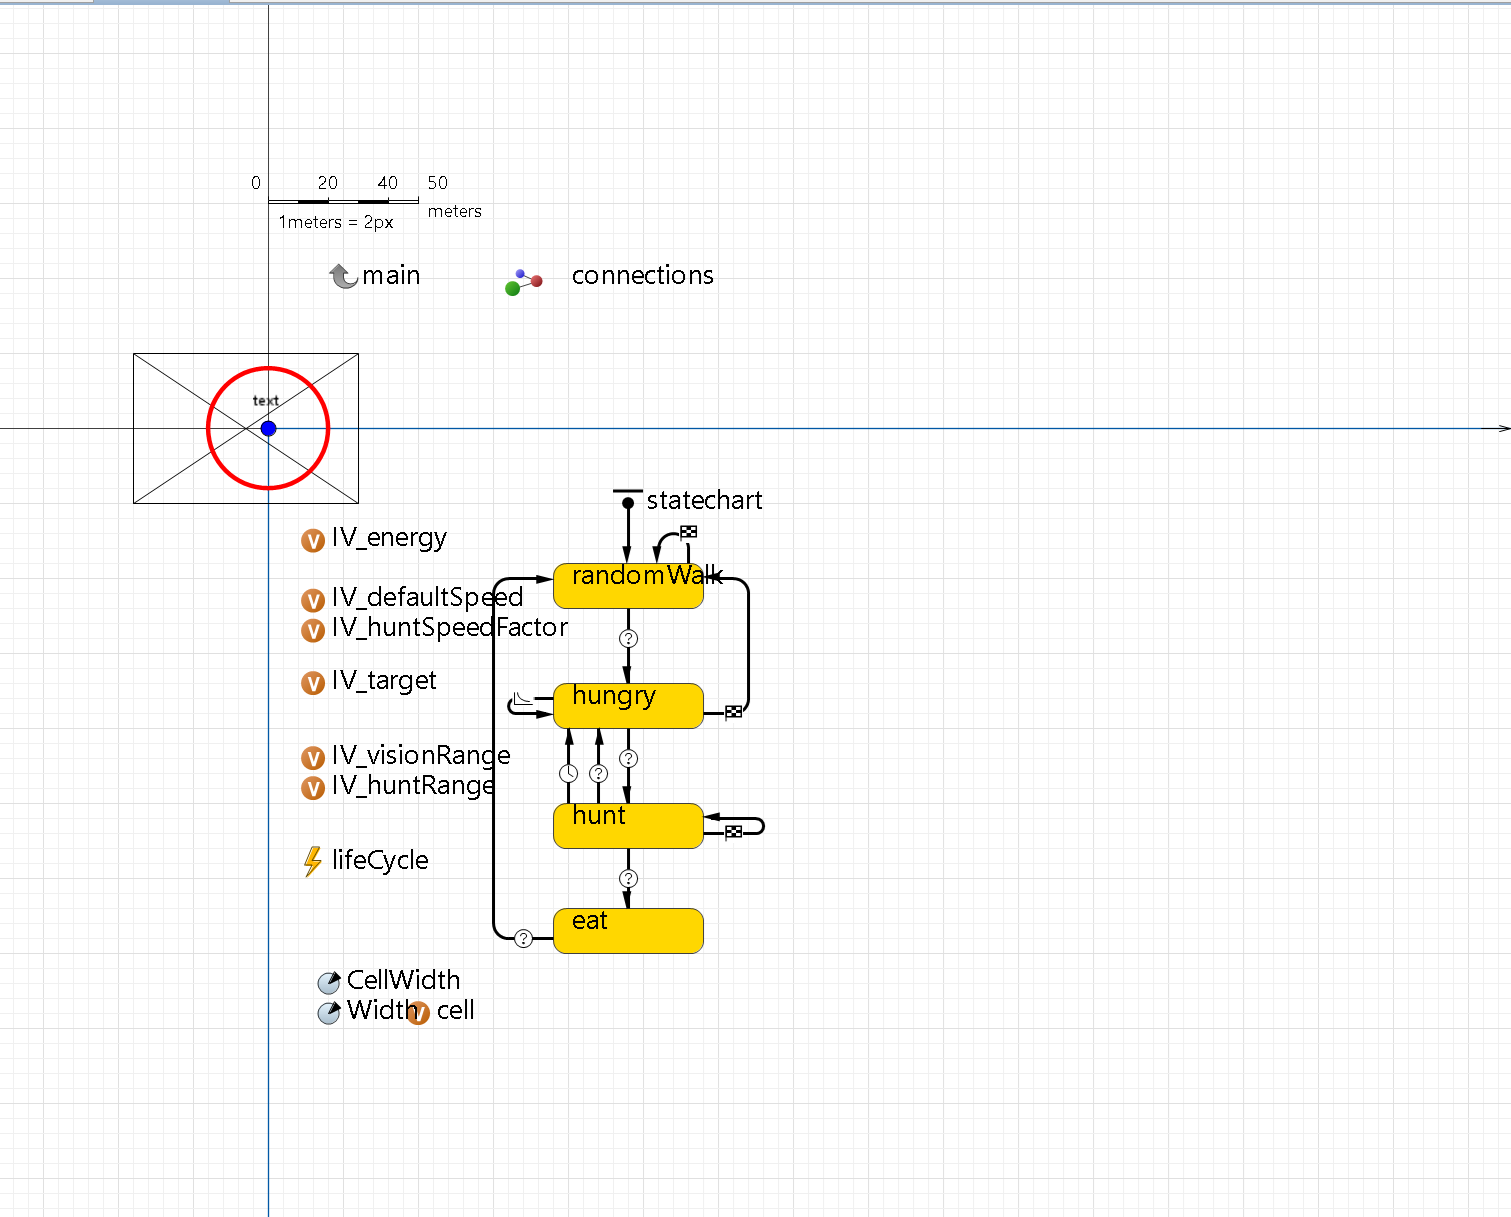
\includegraphics[width=0.9\columnwidth]{A_predator.png}
    \caption{Predator agent statechart}
    \label{fig:predatorAgent}
\end{figure}

\subsubsection{\texttt{A\_Food}}

Food is represented as spatially distributed renewable resources. Fish agents consume food to gain energy, while food regenerates over time, maintaining a dynamic resource landscape.

\subsection{Environment and intervention}

The environment is a continuous 2D space in which all agents interact locally within a perception radius.

The shipwreck is modelled as an environmental event rather than an agent. At time $t = T_w$, the shipwreck introduces three effects:
\begin{itemize}
    \item \textbf{Immediate impact:} fish and food within a radius ($killRadius$) are removed,
    \item \textbf{Pollution:} a surrounding area ($contamRadius$) reduces food availability and increases mortality risk,
    \item \textbf{Shelter:} over time, the wreck provides protection from predators within its vicinity.
\end{itemize}

\subsection{Experimental design}

A behavioural sensitivity analysis is conducted by varying key fish behaviours.

\textbf{Independent variables:}
\begin{itemize}
    \item shelter preference,
    \item schooling tendency.
\end{itemize}

\textbf{Dependent variables:}
\begin{itemize}
    \item fish population size,
    \item survival rate immediately after disturbance,
    \item recovery time to equilibrium.
\end{itemize}

Each experiment is repeated multiple times to account for stochastic variability.

\section{Results and discussion}
figure of the world where everything is included.

-discussion and results compared to plans in before hand, 
-what was implemented
-what changed from before plan

\begin{figure}[h]
    \centering
    \includegraphics[width=0.9\columnwidth]{example-image-a}
    \caption{Example placeholder figure.}
    \label{fig:demo}
\end{figure}


\section{Conclusion}



\balance
\bibliography{Bib.bib}

\end{document}